\documentclass[addpoints,12pt]{exam}
\usepackage{amsmath}
\usepackage{amsthm}
\usepackage{amsfonts}
\usepackage{systeme}
\usepackage{graphicx}
\usepackage{caption}
\usepackage{xfrac}
\usepackage{physics}
\usepackage{microtype}
\usepackage{eulervm}
%\usepackage[framemethod=tikz]{mdframed}
\usepackage{thmtools}
\usepackage{etoolbox}
%\usepackage{fouriernc}
\usepackage{mdframed}
\usepackage[overload]{empheq}
\usepackage{adjustbox}
\usepackage{enumitem}
\usepackage[explicit]{titlesec}
% adds in \varnothing for empty set
\usepackage{amssymb}
% adds in formated SI units
%\usepackage{siunitx}

\pagestyle{headandfoot}
\runningfootrule
\firstpageheadrule
\runningheadrule

\newcommand{\class}{Math 0097}
\newcommand{\sem}{2211}
\newcommand{\due}{}
\newcommand{\sect}{3.3}
\newcommand{\topic}{Slope}

\firstpageheader{\class}{\sect - \topic}{}
\runningheader{\class}{\sect - \topic}{}
\firstpagefooter{\class}{}{Page \thepage\ of \numpages}
\runningfooter{\class}{}{Page \thepage\ of \numpages}

\newif\ifprintselected
\printselectedtrue
%\printselectedfalse

\newenvironment{select}
{\ifprintselected
	\printanswers
	\fi
}
{}

\theoremstyle{definition}
\newtheorem{theorem}{Theorem}
%\newtheorem{example}{Example}[subsection]
%\newtheorem{definition}{Definition}
%\newmdtheoremenv{definition}{Definition}[subsection]
%\newmdtheoremenv{example}{Example}[subsection]
\AtBeginEnvironment{defn}{\begin{minipage}{\textwidth}}
\AtEndEnvironment{defn}{\end{minipage}}
%\AtBeginEnvironment{example}{\begin{minipage}{\textwidth}}
%\AtEndEnvironment{example}{\end{minipage}}
\newcommand{\iu}{{i\mkern1mu}}

\setlength{\gridsize}{5mm}
\setlength{\gridlinewidth}{0.1pt}

\printanswers
\DeclareMathSizes{12}{12}{12}{12}

%%%%%%%%%%%%%%%%%%%%%%%%
% Create bars around subsubsection
%%%%%%%%%%%%%%%%%%%%%%%%

\titleformat{\subsubsection}
   {\large\bfseries}% format
   {}% label
   {0pt}% sep
   {\titlerule \vspace{.1in} #1}% before code
      [{\titlerule[0.4pt]\vspace{.1in}}]% after code
\titlespacing{\subsubsection}
   {0pt}% left
   {0pt}% before sep
   {\baselineskip}% after sep
   
%%%%%%%%%%%%%%%%%%%%%%%
% Create line break after definition label
%%%%%%%%%%%%%%%%%%%%%%%   
\newtheoremstyle{break}
  {\topsep}{\topsep}%
  {}{}%\itshape
  {\bfseries}{}%
  {\newline}{}%
\theoremstyle{break}
\newmdtheoremenv{definition}{Definition}[subsection]
\theoremstyle{break}
\newtheorem{example}{Example}[subsection]

%%%%%%%%%%%%%%%%%%%%%%
% start document
% set section, subsection (use n-1 for sub)
%%%%%%%%%%%%%%%%%%%%%%


\begin{document}
\setcounter{section}{3}
\setcounter{subsection}{2}

\subsection{Slope}

\vspace{.15in}

\begin{definition}[Slope]
\mbox{}\\
\vspace{-.5in}
\begin{itemize}
\item describes the \emph{steepness} of the line
\item defined as $m = \dfrac{\delta y}{\delta x} = \dfrac{\text{rise}}{\text{run}} = \dfrac{y_2-y_1}{x_2-x_1}$
\item describes how quickly one variable changes with respect to another variable
\end{itemize}
\end{definition}

\vspace{.15in}

\begin{example}
Find the slope of the line containing the points $(-3,4)$ and $(-4,-2)$.
\vspace{1in}
\end{example}

\begin{example}
Find the slope of the line containing the points $(4,-2)$ and $(-1,5)$.
\vspace{1in}
\end{example}

\subsubsection*{Horizontal \& Vertical Lines}
\begin{minipage}{.5\textwidth}
\begin{example}
Find the slope of the line\\
containing the points $(5,4)$ and $(3,4)$.
\end{example}
\end{minipage}%
\begin{minipage}{.5\textwidth}
\begin{example}
Find the slope of the line\\
containing the points $(2,5)$ and $(2,1)$.
\end{example}
\end{minipage}%

\newpage

\subsubsection*{Visualizing Slope}
\begin{figure}[h]
\centering
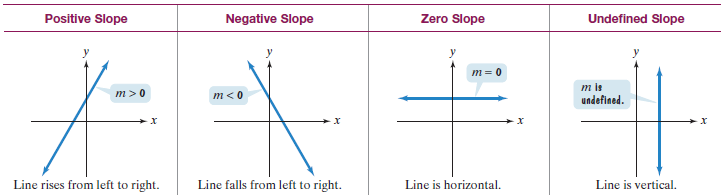
\includegraphics[scale=.8]{../images/types_of_slope}
\end{figure}

\vspace{.15in}

\subsubsection*{Parallel \& Perpendicular Lines}
\vspace{.15in}

\begin{definition}[Parallel Lines]
Two lines that never intersect are said to be parallel. Two parallel lines have the same slope; that is, $m_1 = m_2$.
\end{definition}

\vspace{.15in}

\begin{example}
Show that the line passing through $(4,2)$ and $(6,6)$ is parallel to the line containing the points $(0,-2)$ and $(1,0)$.
\end{example}

\newpage

\begin{definition}[Perpendicular Lines]
If two lines intersect and form a $90\deg$ angle, they are said to be perpendicular. If two lines are perpendicular, then the product of their slopes is $-1$.
\[m_1\cdot m_2 = -1\]
We say that their slopes are \emph{negative reciprocals}.
\end{definition}

\vspace{.15in}

\begin{example}
Show that the line containing the points $(-1,4)$ and $(3,2)$ is perpendicular to the line containing $(-2,-1)$ and $(2,7)$.
\vspace{1.5in}
\end{example}

\begin{example}
In 2000, 11.2 million men lived alone.\\
In 2013, 15 million men lived alone.\\
Find the \emph{average rate of change} and describe what it means.
\end{example}


\end{document}